\documentclass{standalone}
\usepackage{tikz}
\usetikzlibrary{patterns, positioning}
\usepackage[sfdefault]{ClearSans} %% option 'sfdefault' activates Clear Sans as the default text font
\usepackage[T1]{fontenc}

\begin{document}
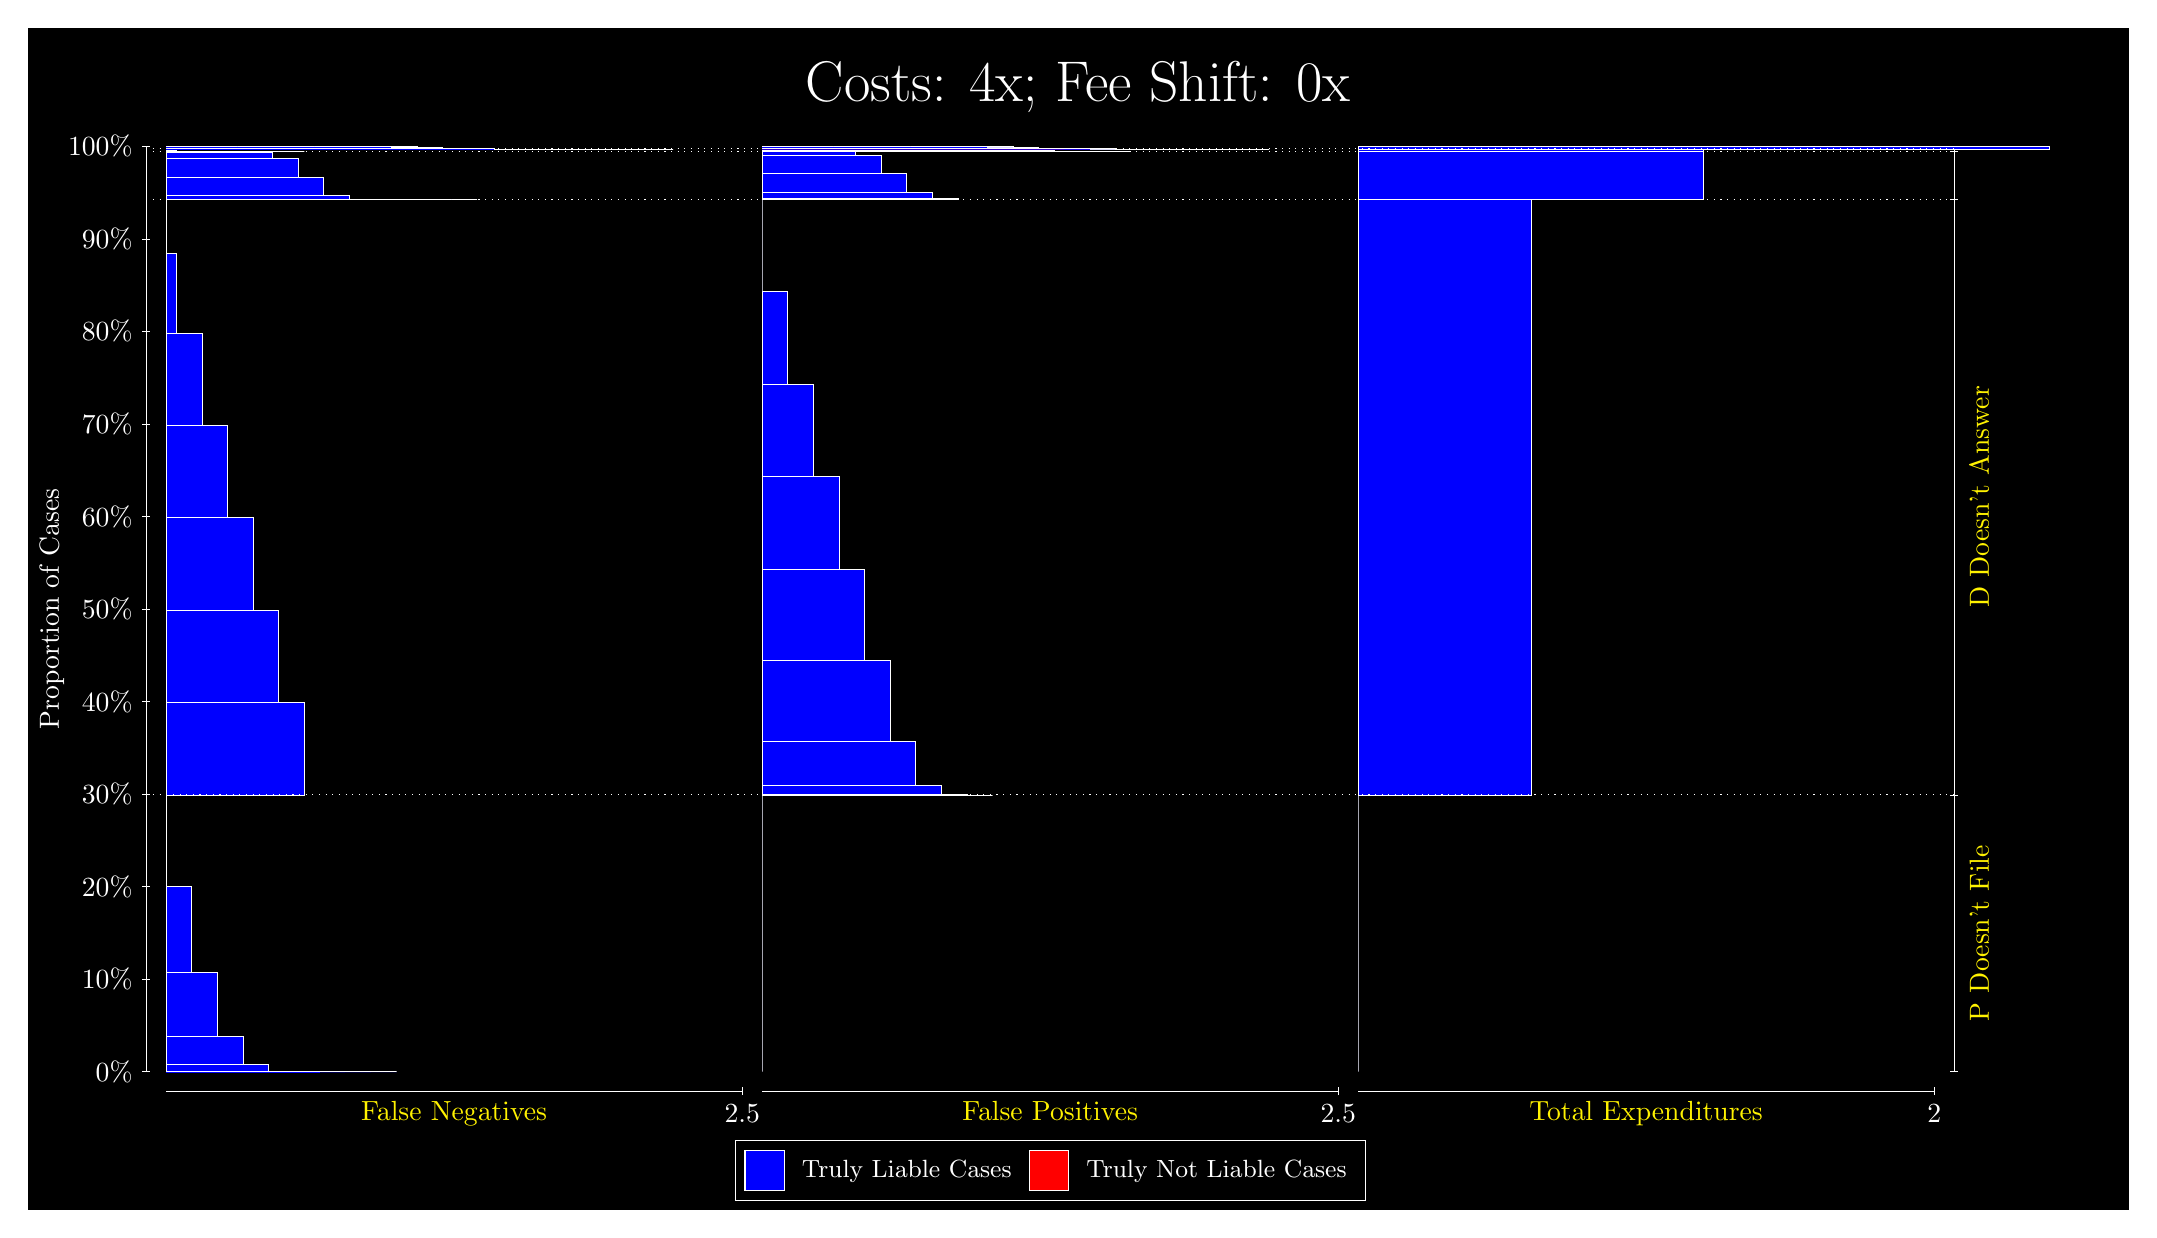
\begin{tikzpicture}
\draw[fill=black] (0,0) rectangle (26.667,15);
\draw[text=white] (0,13.5) rectangle (26.667,15) node[midway] {\huge Costs: 4x; Fee Shift: 0x};
\draw[white, very thin] (1.5,1.75) -- (1.5,13.5);
\node[rotate=90, text=white, anchor=center] at (0.3, 7.625) {Proportion of Cases};
\draw[white, very thin] (1.45,1.75) -- (1.55,1.75);
\node[text=white, anchor=east] at (1.45, 1.75) {0\%};
\draw[white, very thin] (1.45,2.925) -- (1.55,2.925);
\node[text=white, anchor=east] at (1.45, 2.925) {10\%};
\draw[white, very thin] (1.45,4.1) -- (1.55,4.1);
\node[text=white, anchor=east] at (1.45, 4.1) {20\%};
\draw[white, very thin] (1.45,5.275) -- (1.55,5.275);
\node[text=white, anchor=east] at (1.45, 5.275) {30\%};
\draw[white, very thin] (1.45,6.45) -- (1.55,6.45);
\node[text=white, anchor=east] at (1.45, 6.45) {40\%};
\draw[white, very thin] (1.45,7.625) -- (1.55,7.625);
\node[text=white, anchor=east] at (1.45, 7.625) {50\%};
\draw[white, very thin] (1.45,8.8) -- (1.55,8.8);
\node[text=white, anchor=east] at (1.45, 8.8) {60\%};
\draw[white, very thin] (1.45,9.975) -- (1.55,9.975);
\node[text=white, anchor=east] at (1.45, 9.975) {70\%};
\draw[white, very thin] (1.45,11.15) -- (1.55,11.15);
\node[text=white, anchor=east] at (1.45, 11.15) {80\%};
\draw[white, very thin] (1.45,12.325) -- (1.55,12.325);
\node[text=white, anchor=east] at (1.45, 12.325) {90\%};
\draw[white, very thin] (1.45,13.5) -- (1.55,13.5);
\node[text=white, anchor=east] at (1.45, 13.5) {100\%};

\draw[white, very thin] (24.457,1.75) -- (24.457,13.5);
\draw[white, very thin] (24.407,1.75) -- (24.507,1.75);
\node[anchor=west] at (24.407, 1.75) {};
\draw[white, very thin] (24.407,5.264) -- (24.507,5.264);
\node[anchor=west] at (24.407, 5.264) {};
\draw[white, very thin] (24.407,12.829) -- (24.507,12.829);
\node[anchor=west] at (24.407, 12.829) {};
\draw[white, very thin] (24.407,13.437) -- (24.507,13.437);
\node[anchor=west] at (24.407, 13.437) {};
\draw[white, very thin] (24.407,13.467) -- (24.507,13.467);
\node[anchor=west] at (24.407, 13.467) {};
\draw[white, very thin] (24.407,13.5) -- (24.507,13.5);
\node[anchor=west] at (24.407, 13.5) {};

\draw[white, very thin, fill=blue] (1.75,1.75) rectangle (4.6775,1.75);
\draw[white, very thin, fill=blue] (1.75,1.75) rectangle (4.3523,1.75);
\draw[white, very thin, fill=blue] (1.75,1.75) rectangle (4.027,1.75);
\draw[white, very thin, fill=blue] (1.75,1.75) rectangle (3.7017,1.7503);
\draw[white, very thin, fill=blue] (1.75,1.7503) rectangle (3.3764,1.7576);
\draw[white, very thin, fill=blue] (1.75,1.7576) rectangle (3.0511,1.8361);
\draw[white, very thin, fill=blue] (1.75,1.8361) rectangle (2.7258,2.1984);
\draw[white, very thin, fill=blue] (1.75,2.1984) rectangle (2.4006,3.0086);
\draw[white, very thin, fill=blue] (1.75,3.0086) rectangle (2.0753,4.0995);
\draw[white, very thin, fill=red] (1.75,4.0995) rectangle (1.75,4.0995);
\draw[white, very thin, fill=blue] (1.75,4.0995) rectangle (1.75,5.264);
\draw[white, very thin, fill=blue] (1.75,5.264) rectangle (3.5065,6.439);
\draw[white, very thin, fill=blue] (1.75,6.439) rectangle (3.1812,7.614);
\draw[white, very thin, fill=blue] (1.75,7.614) rectangle (2.856,8.789);
\draw[white, very thin, fill=blue] (1.75,8.789) rectangle (2.5307,9.9634);
\draw[white, very thin, fill=blue] (1.75,9.9634) rectangle (2.2054,11.124);
\draw[white, very thin, fill=blue] (1.75,11.124) rectangle (1.8801,12.147);
\draw[white, very thin, fill=red] (1.75,12.147) rectangle (1.75,12.147);
\draw[white, very thin, fill=blue] (1.75,12.147) rectangle (1.75,12.829);
\draw[white, very thin, fill=blue] (1.75,12.829) rectangle (5.7022,12.829);
\draw[white, very thin, fill=blue] (1.75,12.829) rectangle (5.3769,12.829);
\draw[white, very thin, fill=blue] (1.75,12.829) rectangle (5.0516,12.829);
\draw[white, very thin, fill=blue] (1.75,12.829) rectangle (4.7263,12.829);
\draw[white, very thin, fill=blue] (1.75,12.829) rectangle (4.4011,12.831);
\draw[white, very thin, fill=blue] (1.75,12.831) rectangle (4.0758,12.879);
\draw[white, very thin, fill=blue] (1.75,12.879) rectangle (3.7505,13.104);
\draw[white, very thin, fill=blue] (1.75,13.104) rectangle (3.4252,13.349);
\draw[white, very thin, fill=blue] (1.75,13.349) rectangle (3.0999,13.427);
\draw[white, very thin, fill=blue] (1.75,13.427) rectangle (2.7746,13.437);
\draw[white, very thin, fill=red] (1.75,13.437) rectangle (1.75,13.437);
\draw[white, very thin, fill=blue] (1.75,13.437) rectangle (3.5065,13.437);
\draw[white, very thin, fill=blue] (1.75,13.437) rectangle (3.1812,13.437);
\draw[white, very thin, fill=blue] (1.75,13.437) rectangle (2.856,13.437);
\draw[white, very thin, fill=blue] (1.75,13.437) rectangle (2.5307,13.437);
\draw[white, very thin, fill=blue] (1.75,13.437) rectangle (2.2054,13.44);
\draw[white, very thin, fill=blue] (1.75,13.44) rectangle (1.8801,13.453);
\draw[white, very thin, fill=red] (1.75,13.453) rectangle (1.75,13.453);
\draw[white, very thin, fill=blue] (1.75,13.453) rectangle (1.75,13.467);
\draw[white, very thin, fill=blue] (1.75,13.467) rectangle (8.1906,13.467);
\draw[white, very thin, fill=blue] (1.75,13.467) rectangle (7.8653,13.467);
\draw[white, very thin, fill=blue] (1.75,13.467) rectangle (7.54,13.467);
\draw[white, very thin, fill=blue] (1.75,13.467) rectangle (7.54,13.467);
\draw[white, very thin, fill=blue] (1.75,13.467) rectangle (7.2148,13.467);
\draw[white, very thin, fill=blue] (1.75,13.467) rectangle (6.8895,13.467);
\draw[white, very thin, fill=blue] (1.75,13.467) rectangle (6.5642,13.467);
\draw[white, very thin, fill=blue] (1.75,13.467) rectangle (6.2389,13.468);
\draw[white, very thin, fill=blue] (1.75,13.468) rectangle (5.9136,13.469);
\draw[white, very thin, fill=blue] (1.75,13.469) rectangle (5.9136,13.472);
\draw[white, very thin, fill=blue] (1.75,13.472) rectangle (5.5883,13.478);
\draw[white, very thin, fill=blue] (1.75,13.478) rectangle (5.5883,13.479);
\draw[white, very thin, fill=blue] (1.75,13.479) rectangle (5.2631,13.488);
\draw[white, very thin, fill=blue] (1.75,13.488) rectangle (4.9378,13.489);
\draw[white, very thin, fill=blue] (1.75,13.489) rectangle (4.9378,13.495);
\draw[white, very thin, fill=blue] (1.75,13.495) rectangle (4.6125,13.495);
\draw[white, very thin, fill=blue] (1.75,13.495) rectangle (4.6125,13.497);
\draw[white, very thin, fill=blue] (1.75,13.497) rectangle (4.6125,13.498);
\draw[white, very thin, fill=blue] (1.75,13.498) rectangle (4.2872,13.499);
\draw[white, very thin, fill=blue] (1.75,13.499) rectangle (4.2872,13.5);
\draw[white, very thin, fill=blue] (1.75,13.5) rectangle (3.9619,13.5);
\draw[white, very thin, fill=blue] (1.75,13.5) rectangle (3.6366,13.5);
\draw[white, very thin, fill=blue] (1.75,13.5) rectangle (3.3114,13.5);
\draw[white, very thin, fill=blue] (1.75,13.5) rectangle (3.3114,13.5);
\draw[white, very thin, fill=blue] (1.75,13.5) rectangle (2.9861,13.5);
\draw[white, very thin, fill=blue] (1.75,13.5) rectangle (2.9861,13.5);
\draw[white, very thin, fill=blue] (1.75,13.5) rectangle (2.6608,13.5);
\draw[white, very thin, fill=blue] (1.75,13.5) rectangle (2.6608,13.5);
\draw[white, very thin, fill=blue] (1.75,13.5) rectangle (2.3355,13.5);
\draw[white, very thin, fill=red] (1.75,13.5) rectangle (1.75,13.5);
\draw[white, very thin, fill=red] (9.3189,1.75) rectangle (9.3189,1.75);
\draw[white, very thin, fill=blue] (9.3189,1.75) rectangle (9.3189,5.264);
\draw[white, very thin, fill=red] (9.3189,5.264) rectangle (12.246,5.264);
\draw[white, very thin, fill=blue] (9.3189,5.264) rectangle (12.246,5.264);
\draw[white, very thin, fill=blue] (9.3189,5.264) rectangle (11.921,5.2701);
\draw[white, very thin, fill=blue] (9.3189,5.2701) rectangle (11.596,5.3833);
\draw[white, very thin, fill=blue] (9.3189,5.3833) rectangle (11.271,5.9454);
\draw[white, very thin, fill=blue] (9.3189,5.9454) rectangle (10.945,6.9686);
\draw[white, very thin, fill=blue] (9.3189,6.9686) rectangle (10.62,8.1291);
\draw[white, very thin, fill=blue] (9.3189,8.1291) rectangle (10.295,9.3035);
\draw[white, very thin, fill=blue] (9.3189,9.3035) rectangle (9.9694,10.479);
\draw[white, very thin, fill=blue] (9.3189,10.479) rectangle (9.6442,11.654);
\draw[white, very thin, fill=blue] (9.3189,11.654) rectangle (9.3189,12.829);
\draw[white, very thin, fill=red] (9.3189,12.829) rectangle (11.807,12.829);
\draw[white, very thin, fill=blue] (9.3189,12.829) rectangle (11.807,12.839);
\draw[white, very thin, fill=blue] (9.3189,12.839) rectangle (11.482,12.917);
\draw[white, very thin, fill=blue] (9.3189,12.917) rectangle (11.157,13.162);
\draw[white, very thin, fill=blue] (9.3189,13.162) rectangle (10.831,13.387);
\draw[white, very thin, fill=blue] (9.3189,13.387) rectangle (10.506,13.435);
\draw[white, very thin, fill=blue] (9.3189,13.435) rectangle (10.181,13.437);
\draw[white, very thin, fill=blue] (9.3189,13.437) rectangle (9.8556,13.437);
\draw[white, very thin, fill=blue] (9.3189,13.437) rectangle (9.5303,13.437);
\draw[white, very thin, fill=blue] (9.3189,13.437) rectangle (9.3189,13.437);
\draw[white, very thin, fill=red] (9.3189,13.437) rectangle (14.003,13.437);
\draw[white, very thin, fill=blue] (9.3189,13.437) rectangle (14.003,13.437);
\draw[white, very thin, fill=blue] (9.3189,13.437) rectangle (13.678,13.437);
\draw[white, very thin, fill=blue] (9.3189,13.437) rectangle (13.352,13.439);
\draw[white, very thin, fill=blue] (9.3189,13.439) rectangle (13.027,13.451);
\draw[white, very thin, fill=blue] (9.3189,13.451) rectangle (12.702,13.464);
\draw[white, very thin, fill=blue] (9.3189,13.464) rectangle (12.377,13.467);
\draw[white, very thin, fill=blue] (9.3189,13.467) rectangle (12.051,13.467);
\draw[white, very thin, fill=blue] (9.3189,13.467) rectangle (11.726,13.467);
\draw[white, very thin, fill=blue] (9.3189,13.467) rectangle (11.401,13.467);
\draw[white, very thin, fill=blue] (9.3189,13.467) rectangle (11.075,13.467);
\draw[white, very thin, fill=red] (9.3189,13.467) rectangle (15.759,13.467);
\draw[white, very thin, fill=blue] (9.3189,13.467) rectangle (15.759,13.467);
\draw[white, very thin, fill=blue] (9.3189,13.467) rectangle (15.434,13.467);
\draw[white, very thin, fill=red] (9.3189,13.467) rectangle (15.434,13.467);
\draw[white, very thin, fill=blue] (9.3189,13.467) rectangle (15.434,13.467);
\draw[white, very thin, fill=red] (9.3189,13.467) rectangle (15.109,13.467);
\draw[white, very thin, fill=blue] (9.3189,13.467) rectangle (15.109,13.467);
\draw[white, very thin, fill=blue] (9.3189,13.467) rectangle (15.109,13.467);
\draw[white, very thin, fill=blue] (9.3189,13.467) rectangle (14.784,13.467);
\draw[white, very thin, fill=red] (9.3189,13.467) rectangle (14.784,13.467);
\draw[white, very thin, fill=blue] (9.3189,13.467) rectangle (14.784,13.467);
\draw[white, very thin, fill=blue] (9.3189,13.467) rectangle (14.784,13.467);
\draw[white, very thin, fill=blue] (9.3189,13.467) rectangle (14.458,13.467);
\draw[white, very thin, fill=red] (9.3189,13.467) rectangle (14.458,13.467);
\draw[white, very thin, fill=blue] (9.3189,13.467) rectangle (14.458,13.467);
\draw[white, very thin, fill=blue] (9.3189,13.467) rectangle (14.458,13.467);
\draw[white, very thin, fill=blue] (9.3189,13.467) rectangle (14.133,13.467);
\draw[white, very thin, fill=red] (9.3189,13.467) rectangle (14.133,13.467);
\draw[white, very thin, fill=blue] (9.3189,13.467) rectangle (14.133,13.467);
\draw[white, very thin, fill=blue] (9.3189,13.467) rectangle (14.133,13.467);
\draw[white, very thin, fill=blue] (9.3189,13.467) rectangle (13.808,13.467);
\draw[white, very thin, fill=blue] (9.3189,13.467) rectangle (13.808,13.468);
\draw[white, very thin, fill=red] (9.3189,13.468) rectangle (13.808,13.468);
\draw[white, very thin, fill=blue] (9.3189,13.468) rectangle (13.808,13.469);
\draw[white, very thin, fill=blue] (9.3189,13.469) rectangle (13.808,13.469);
\draw[white, very thin, fill=blue] (9.3189,13.469) rectangle (13.482,13.469);
\draw[white, very thin, fill=blue] (9.3189,13.469) rectangle (13.482,13.472);
\draw[white, very thin, fill=red] (9.3189,13.472) rectangle (13.482,13.472);
\draw[white, very thin, fill=blue] (9.3189,13.472) rectangle (13.482,13.472);
\draw[white, very thin, fill=blue] (9.3189,13.472) rectangle (13.157,13.472);
\draw[white, very thin, fill=red] (9.3189,13.472) rectangle (13.157,13.472);
\draw[white, very thin, fill=blue] (9.3189,13.472) rectangle (13.157,13.478);
\draw[white, very thin, fill=blue] (9.3189,13.478) rectangle (13.157,13.479);
\draw[white, very thin, fill=blue] (9.3189,13.479) rectangle (12.832,13.479);
\draw[white, very thin, fill=red] (9.3189,13.479) rectangle (12.832,13.479);
\draw[white, very thin, fill=blue] (9.3189,13.479) rectangle (12.832,13.487);
\draw[white, very thin, fill=blue] (9.3189,13.487) rectangle (12.832,13.488);
\draw[white, very thin, fill=blue] (9.3189,13.488) rectangle (12.507,13.489);
\draw[white, very thin, fill=blue] (9.3189,13.489) rectangle (12.507,13.495);
\draw[white, very thin, fill=blue] (9.3189,13.495) rectangle (12.507,13.495);
\draw[white, very thin, fill=blue] (9.3189,13.495) rectangle (12.181,13.497);
\draw[white, very thin, fill=blue] (9.3189,13.497) rectangle (12.181,13.497);
\draw[white, very thin, fill=blue] (9.3189,13.497) rectangle (12.181,13.499);
\draw[white, very thin, fill=blue] (9.3189,13.499) rectangle (11.856,13.5);
\draw[white, very thin, fill=blue] (9.3189,13.5) rectangle (11.856,13.5);
\draw[white, very thin, fill=blue] (9.3189,13.5) rectangle (11.856,13.5);
\draw[white, very thin, fill=blue] (9.3189,13.5) rectangle (11.531,13.5);
\draw[white, very thin, fill=blue] (9.3189,13.5) rectangle (11.531,13.5);
\draw[white, very thin, fill=blue] (9.3189,13.5) rectangle (11.206,13.5);
\draw[white, very thin, fill=blue] (9.3189,13.5) rectangle (11.206,13.5);
\draw[white, very thin, fill=blue] (9.3189,13.5) rectangle (11.206,13.5);
\draw[white, very thin, fill=blue] (9.3189,13.5) rectangle (10.88,13.5);
\draw[white, very thin, fill=blue] (9.3189,13.5) rectangle (10.88,13.5);
\draw[white, very thin, fill=blue] (9.3189,13.5) rectangle (10.555,13.5);
\draw[white, very thin, fill=blue] (9.3189,13.5) rectangle (10.555,13.5);
\draw[white, very thin, fill=blue] (9.3189,13.5) rectangle (10.555,13.5);
\draw[white, very thin, fill=blue] (9.3189,13.5) rectangle (10.23,13.5);
\draw[white, very thin, fill=blue] (9.3189,13.5) rectangle (9.9044,13.5);
\draw[white, very thin, fill=red] (16.888,1.75) rectangle (16.888,1.75);
\draw[white, very thin, fill=blue] (16.888,1.75) rectangle (16.888,5.264);
\draw[white, very thin, fill=red] (16.888,5.264) rectangle (19.083,5.264);
\draw[white, very thin, fill=blue] (16.888,5.264) rectangle (19.083,12.829);
\draw[white, very thin, fill=red] (16.888,12.829) rectangle (21.279,12.829);
\draw[white, very thin, fill=blue] (16.888,12.829) rectangle (21.279,13.437);
\draw[white, very thin, fill=red] (16.888,13.437) rectangle (21.279,13.437);
\draw[white, very thin, fill=blue] (16.888,13.437) rectangle (21.279,13.467);
\draw[white, very thin, fill=red] (16.888,13.467) rectangle (25.67,13.467);
\draw[white, very thin, fill=blue] (16.888,13.467) rectangle (25.67,13.467);
\draw[white, very thin, fill=red] (16.888,13.467) rectangle (25.67,13.467);
\draw[white, very thin, fill=blue] (16.888,13.467) rectangle (25.67,13.5);
\draw[white, very thin, fill=red] (16.888,13.5) rectangle (25.67,13.5);
\draw[white, very thin, fill=blue] (16.888,13.5) rectangle (25.67,13.5);
\draw[white, dotted] (1.5,5.264) -- (24.457,5.264);
\draw[white, dotted] (1.5,12.829) -- (24.457,12.829);
\draw[white, dotted] (1.5,13.437) -- (24.457,13.437);
\draw[white, dotted] (1.5,13.467) -- (24.457,13.467);
\draw[white, very thin] (1.75,1.5) -- (9.0689,1.5);
\node[text=yellow, anchor=north] at (5.4094, 1.5) {False Negatives};
\draw[white, very thin] (9.0689,1.45) -- (9.0689,1.55);
\node[text=white, anchor=north] at (9.0689, 1.45) {2.5};

\draw[white, very thin] (9.3189,1.5) -- (16.638,1.5);
\node[text=yellow, anchor=north] at (12.978, 1.5) {False Positives};
\draw[white, very thin] (16.638,1.45) -- (16.638,1.55);
\node[text=white, anchor=north] at (16.638, 1.45) {2.5};

\draw[white, very thin] (16.888,1.5) -- (24.207,1.5);
\node[text=yellow, anchor=north] at (20.547, 1.5) {Total Expenditures};
\draw[white, very thin] (24.207,1.45) -- (24.207,1.55);
\node[text=white, anchor=north] at (24.207, 1.45) {2};

\node[text=yellow, centered, rotate=90] at (24.777, 3.507) {P Doesn't File};
\node[text=yellow, centered, rotate=90] at (24.777, 9.0463) {D Doesn't Answer};




\draw (12.978300999999998,1.5) node[draw=none] (baseCoordinate) {};
\begin{scope}[align=center]
        \matrix[scale=0.5, draw=white, below=0.5cm of baseCoordinate, nodes={draw}, column sep=0.1cm]{
            \node[rectangle, draw, minimum width=0.5cm, minimum height=0.5cm, fill=blue] {}; &
            \node[draw=none, font=\small, text=white] (B) {Truly Liable Cases}; &
            \node[rectangle, draw, minimum width=0.5cm, minimum height=0.5cm, fill=red] {}; &
            \node[draw=none, font=\small, text=white] (B) {Truly Not Liable Cases}; \\
            };
\end{scope}

\end{tikzpicture}
\end{document}